\documentclass[11pt,a4paper]{article}

% ── Paquetes ──────────────────────────────────────────────────────────
\usepackage[utf8]{inputenc}
\usepackage[T1]{fontenc}
\usepackage[spanish]{babel}
\usepackage{geometry}
\geometry{left=2.5cm, right=2.5cm, top=2.5cm, bottom=2.5cm}
\usepackage{graphicx}
\usepackage{listings}
\usepackage{xcolor}
\usepackage{hyperref}
\usepackage{fancyhdr}
\usepackage{titlesec}
\usepackage{enumitem}
\usepackage{amsmath}
\usepackage{float}
\usepackage{tcolorbox}
\tcbuselibrary{listings,skins}

\setlength{\headheight}{14pt}
\addtolength{\topmargin}{-2pt}

% ── Colores ───────────────────────────────────────────────────────────
\definecolor{codegreen}{rgb}{0.25,0.49,0.18}
\definecolor{codegray}{rgb}{0.5,0.5,0.5}
\definecolor{codepurple}{rgb}{0.58,0,0.82}
\definecolor{backcolour}{rgb}{0.96,0.96,0.96}
\definecolor{keywordblue}{rgb}{0.0,0.0,0.7}
\definecolor{consolebg}{HTML}{1E1E2E}
\definecolor{consolefg}{HTML}{CDD6F4}

% ── Estilo Java ───────────────────────────────────────────────────────
\lstdefinestyle{javastyle}{
    backgroundcolor=\color{backcolour},
    commentstyle=\color{codegreen}\itshape,
    keywordstyle=\color{keywordblue}\bfseries,
    numberstyle=\tiny\color{codegray},
    stringstyle=\color{codepurple},
    basicstyle=\ttfamily\footnotesize,
    breakatwhitespace=false,
    breaklines=true,
    captionpos=b,
    keepspaces=true,
    numbers=left,
    numbersep=5pt,
    showspaces=false,
    showstringspaces=false,
    showtabs=false,
    tabsize=4,
    language=Java,
    frame=single,
    rulecolor=\color{codegray},
    literate={á}{{\'a}}1 {é}{{\'e}}1 {í}{{\'i}}1 {ó}{{\'o}}1 {ú}{{\'u}}1
             {ñ}{{\~n}}1 {Á}{{\'A}}1 {É}{{\'E}}1 {Í}{{\'I}}1 {Ó}{{\'O}}1
             {Ú}{{\'U}}1 {Ñ}{{\~N}}1 {¿}{{\textquestiondown}}1
}
\lstset{style=javastyle}

% ── Encabezado y pie de página ────────────────────────────────────────
\pagestyle{fancy}
\fancyhf{}
\lhead{UNAL — POO}
\rhead{Actividad 1: Algoritmos y Lógica de Programación}
\cfoot{\thepage}
\renewcommand{\headrulewidth}{0.4pt}

% ── Hipervínculos ─────────────────────────────────────────────────────
\hypersetup{
    colorlinks=true,
    linkcolor=blue,
    urlcolor=blue,
    citecolor=blue
}

% ══════════════════════════════════════════════════════════════════════
\begin{document}

% ── Portada ───────────────────────────────────────────────────────────
\begin{center}
    {\Large \textbf{UNIVERSIDAD NACIONAL DE COLOMBIA}} \\[4pt]
    {\large \textbf{Facultad de Ingeniería — Departamento de Ciencias de la Computación}} \\[6pt]
    {\LARGE \textbf{Programación Orientada a Objetos — Actividad 1}} \\[8pt]
    {\large \textbf{Docente:}} Walter Hugo Arboleda \\[6pt]
    {\large \textbf{Autor:}} \\[2pt]
    {\large Cristian Ruiz Hernandez} \hfill \texttt{cruizh@unal.edu.co} \\[4pt]
    {\large \textbf{Repositorio en GitHub:}} \url{https://github.com/cioranemil/trabajo-1}
\end{center}

\vspace{0.2cm}
\hrule
\vspace{0.4cm}

% ── Menú Principal Interactivo ────────────────────────────────────────
\section*{Interfaz Gráfica Principal (Swing GUI)}

Se implementó una interfaz gráfica completa en Java Swing estructurada en un Menú Principal con 5 botones que permiten ejecutar y probar de forma interactiva cada uno de los 5 ejercicios de Lógica de Programación de Efraín Oviedo.

\begin{figure}[H]
\centering
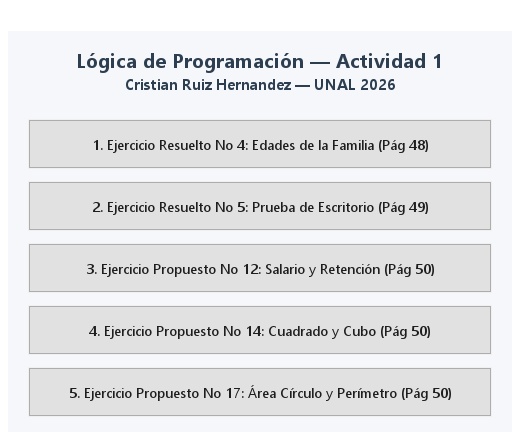
\includegraphics[width=0.75\textwidth]{images/gui_menu_principal.png}
\caption{Menú Principal Interactivo de la Actividad 1.}
\end{figure}

---

% ══════════════════════════════════════════════════════════════════════
\section{Ejercicio Resuelto No 4: Edades de la Familia (Páginas 48 – 49)}

\subsection{Enunciado}
A la mamá de Juan le preguntan su edad, y contesta: tengo 3 hijos, pregúntele a Juan su edad. Alberto tiene $2/3$ de la edad de Juan, Ana tiene $4/3$ de la edad de Juan y mi edad es la suma de las tres. Hacer un algoritmo que muestre la edad de los cuatro.

\subsection{Captura de la Interfaz Visual}
\begin{figure}[H]
\centering
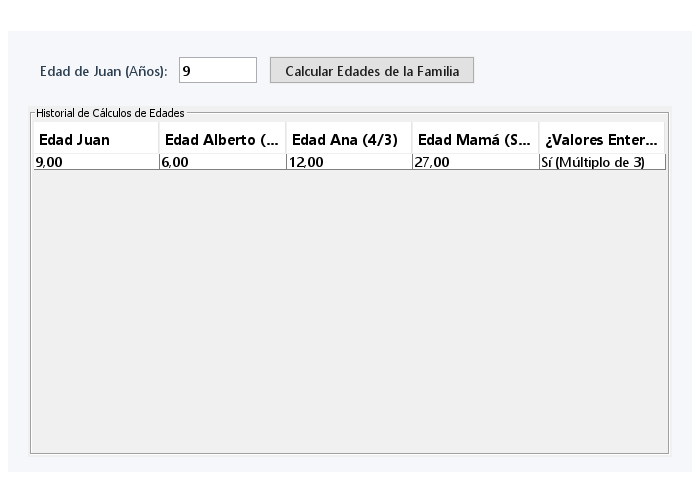
\includegraphics[width=0.82\textwidth]{images/gui_ejercicio_resuelto_4.png}
\caption{Interfaz gráfica interactiva para el Ejercicio Resuelto No 4.}
\end{figure}

\subsection{Diagrama de clases UML}
\begin{tcolorbox}[colframe=blue!60!black,colback=blue!5!white,arc=4mm,title=\textbf{namespace Actividad1.EjercicioResuelto4}]
\centering
\begin{verbatim}
+-------------------------------------------------------------+
|                     EjercicioResuelto4                      |
+-------------------------------------------------------------+
| - edadJuan: double                                          |
| - edadAlberto: double                                       |
| - edadAna: double                                           |
| - edadMama: double                                          |
+-------------------------------------------------------------+
| + EjercicioResuelto4(edadJuan: double)                      |
| + getEdadJuan(): double, getEdadAlberto(): double           |
| + getEdadAna(): double, getEdadMama(): double               |
| + esEdadExacta(): boolean                                   |
| + imprimir(): void                                          |
+-------------------------------------------------------------+
\end{verbatim}
\end{tcolorbox}

\subsection{Casos de uso}
\begin{itemize}[leftmargin=*]
    \item \textbf{Caso de Uso 1: Cálculo de Edades de la Familia}
    \begin{itemize}
        \item \textbf{Actor:} Usuario.
        \item \textbf{Precondición:} La ventana del Ejercicio Resuelto No 4 está abierta.
        \item \textbf{Flujo Principal:} El usuario escribe la edad de Juan (ej: $9$) y presiona \textit{Calcular Edades de la Familia}. El sistema calcula la edad de Alberto ($2/3$), la de Ana ($4/3$) y la de la Mamá (suma), renderizándolas en la tabla \texttt{JTable}.
        \item \textbf{Flujo Alternativo (Formato No Numérico):} Si se ingresa una edad menor o igual a cero o texto, se muestra un diálogo de error impidiendo el cálculo.
    \end{itemize}
\end{itemize}

---

% ══════════════════════════════════════════════════════════════════════
\section{Ejercicio Resuelto No 5: Prueba de Escritorio (Páginas 49 – 50)}

\subsection{Enunciado}
Hacer un seguimiento (prueba de escritorio) del siguiente grupo de instrucciones:
\begin{lstlisting}[language=Java]
INICIO
  SUMA = 0
  X = 20
  SUMA = SUMA + X
  Y = 40
  X = X + Y ** 2
  SUMA = SUMA + X / Y
  ESCRIBA: "EL VALOR DE LA SUMA ES:", SUMA
FIN_INICIO
\end{lstlisting}

\subsection{Captura de la Interfaz Visual}
\begin{figure}[H]
\centering
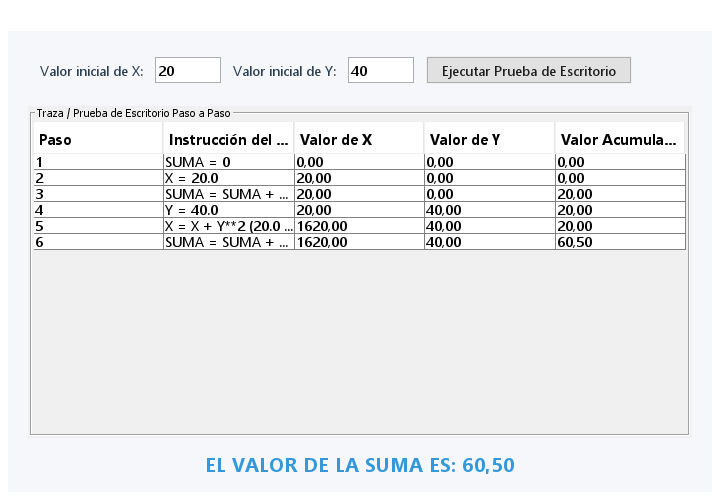
\includegraphics[width=0.82\textwidth]{images/gui_ejercicio_resuelto_5.png}
\caption{Interfaz gráfica interactiva para el Ejercicio Resuelto No 5 (Prueba de Escritorio).}
\end{figure}

\subsection{Diagrama de clases UML}
\begin{tcolorbox}[colframe=blue!60!black,colback=blue!5!white,arc=4mm,title=\textbf{namespace Actividad1.EjercicioResuelto5}]
\centering
\begin{verbatim}
+-------------------------------------------------------------+
|                     EjercicioResuelto5                      |
+-------------------------------------------------------------+
| - suma: double, x: double, y: double                        |
| - pasos: List<PasoPruebaEscritorio>                         |
+-------------------------------------------------------------+
| + EjercicioResuelto5(), EjercicioResuelto5(x:double,y:double)|
| - ejecutarPruebaEscritorio(x:double, y:double): void        |
| + getSumaFinal(): double, getPasos(): List                  |
+-------------------------------------------------------------+
\end{verbatim}
\end{tcolorbox}

\subsection{Casos de uso}
\begin{itemize}[leftmargin=*]
    \item \textbf{Caso de Uso 2: Seguimiento de Prueba de Escritorio Paso a Paso}
    \begin{itemize}
        \item \textbf{Actor:} Usuario / Estudiante.
        \item \textbf{Precondición:} La ventana del Ejercicio Resuelto No 5 está desplegada.
        \item \textbf{Flujo Principal:} El usuario presiona \textit{Ejecutar Prueba de Escritorio}. El sistema evalúa secuencialmente cada instrucción, registra la traza de las variables $X, Y, SUMA$ en una \texttt{JTable} y muestra la suma final ($60.50$).
    \end{itemize}
\end{itemize}

---

% ══════════════════════════════════════════════════════════════════════
\section{Ejercicio Propuesto No 12: Salario y Retención (Página 50)}

\subsection{Enunciado}
Un empleado trabaja 48 horas en la semana a razón de \$5.000 hora. El porcentaje de retención en la fuente es del 12.5\% del salario bruto. Se desea saber cuál es el salario bruto, la retención en la fuente y el salario neto del trabajador.

\subsection{Captura de la Interfaz Visual}
\begin{figure}[H]
\centering
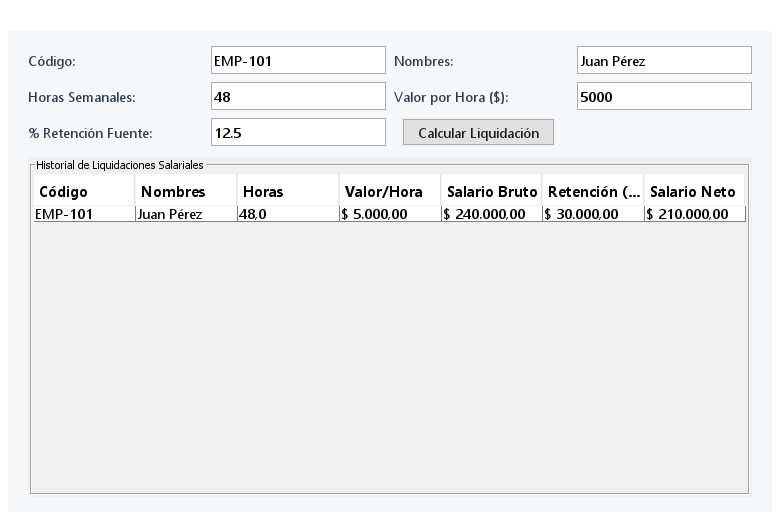
\includegraphics[width=0.82\textwidth]{images/gui_ejercicio_propuesto_12.png}
\caption{Interfaz gráfica interactiva para el Ejercicio Propuesto No 12 (Liquidación Salarial).}
\end{figure}

\subsection{Diagrama de clases UML}
\begin{tcolorbox}[colframe=blue!60!black,colback=blue!5!white,arc=4mm,title=\textbf{namespace Actividad1.EjercicioPropuesto12}]
\centering
\begin{verbatim}
+-------------------------------------------------------------+
|                    EjercicioPropuesto12                     |
+-------------------------------------------------------------+
| - codigoEmpleado: String, nombres: String                   |
| - horasTrabajadas: double, valorHora: double                |
| - porcentajeRetencion: double, salarioBruto: double         |
| - retencionFuente: double, salarioNeto: double              |
+-------------------------------------------------------------+
| + EjercicioPropuesto12()                                    |
| + EjercicioPropuesto12(cod, nom, horas, vHora, retencion)   |
| + getSalarioBruto(): double, getSalarioNeto(): double       |
| + formatoMoneda(valor: double): String                      |
+-------------------------------------------------------------+
\end{verbatim}
\end{tcolorbox}

\subsection{Casos de uso}
\begin{itemize}[leftmargin=*]
    \item \textbf{Caso de Uso 3: Liquidación de Salario Bruto, Retención y Salario Neto}
    \begin{itemize}
        \item \textbf{Actor:} Usuario / Administrador.
        \item \textbf{Precondición:} La ventana del Ejercicio Propuesto No 12 está abierta.
        \item \textbf{Flujo Principal:} El usuario escribe horas, valor por hora y porcentaje de retención, o presiona \textit{Cargar Datos del Libro}. El sistema calcula: $SalarioBruto = 48 \cdot 5000 = \$240.000$, $Retencion = \$240.000 \cdot 12.5\% = \$30.000$, y $SalarioNeto = \$210.000$.
    \end{itemize}
\end{itemize}

---

% ══════════════════════════════════════════════════════════════════════
\section{Ejercicio Propuesto No 14: Cuadrado y Cubo (Página 50)}

\subsection{Enunciado}
Elaborar un algoritmo que lea un número y obtenga su cuadrado y su cubo.

\subsection{Captura de la Interfaz Visual}
\begin{figure}[H]
\centering
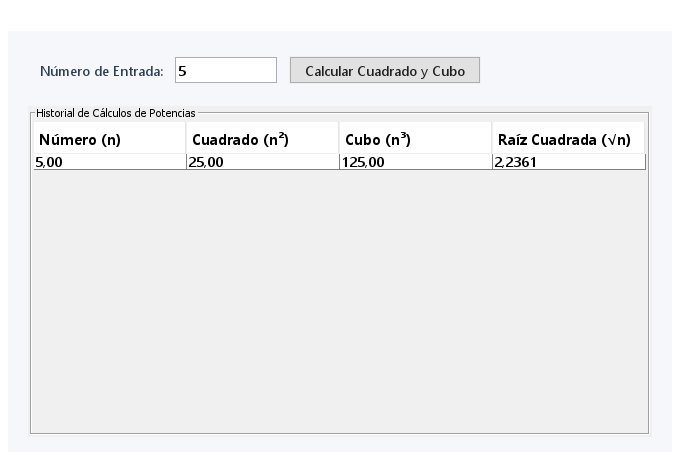
\includegraphics[width=0.82\textwidth]{images/gui_ejercicio_propuesto_14.png}
\caption{Interfaz gráfica interactiva para el Ejercicio Propuesto No 14.}
\end{figure}

\subsection{Diagrama de clases UML}
\begin{tcolorbox}[colframe=blue!60!black,colback=blue!5!white,arc=4mm,title=\textbf{namespace Actividad1.EjercicioPropuesto14}]
\centering
\begin{verbatim}
+-------------------------------------------------------------+
|                    EjercicioPropuesto14                     |
+-------------------------------------------------------------+
| - numero: double, cuadrado: double, cubo: double            |
+-------------------------------------------------------------+
| + EjercicioPropuesto14(numero: double)                      |
| + getCuadrado(): double, getCubo(): double                  |
| + getRaizCuadrada(): double                                 |
+-------------------------------------------------------------+
\end{verbatim}
\end{tcolorbox}

\subsection{Casos de uso}
\begin{itemize}[leftmargin=*]
    \item \textbf{Caso de Uso 4: Cálculo de Potencias (Cuadrado y Cubo)}
    \begin{itemize}
        \item \textbf{Actor:} Usuario.
        \item \textbf{Flujo Principal:} El usuario escribe un número $n$ y presiona \textit{Calcular Cuadrado y Cubo}. El sistema procesa $n^2$ y $n^3$, añadiéndolos a la tabla.
    \end{itemize}
\end{itemize}

---

% ══════════════════════════════════════════════════════════════════════
\section{Ejercicio Propuesto No 17: Círculo y Circunferencia (Página 50)}

\subsection{Enunciado}
Dado el radio de un círculo. Haga un algoritmo que obtenga el área del círculo y la longitud de la circunferencia.

\subsection{Captura de la Interfaz Visual}
\begin{figure}[H]
\centering
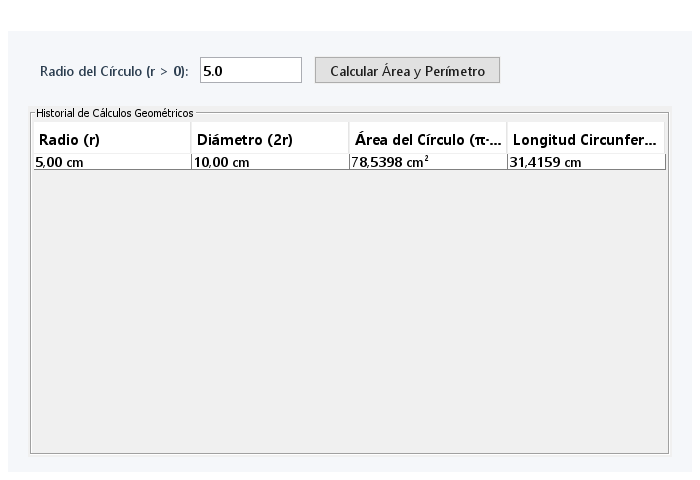
\includegraphics[width=0.82\textwidth]{images/gui_ejercicio_propuesto_17.png}
\caption{Interfaz gráfica interactiva para el Ejercicio Propuesto No 17.}
\end{figure}

\subsection{Diagrama de clases UML}
\begin{tcolorbox}[colframe=blue!60!black,colback=blue!5!white,arc=4mm,title=\textbf{namespace Actividad1.EjercicioPropuesto17}]
\centering
\begin{verbatim}
+-------------------------------------------------------------+
|                    EjercicioPropuesto17                     |
+-------------------------------------------------------------+
| - radio: double, area: double, longitudCircunferencia: d    |
+-------------------------------------------------------------+
| + EjercicioPropuesto17(radio: double)                       |
| + getArea(): double, getLongitudCircunferencia(): double    |
| + getDiametro(): double                                     |
+-------------------------------------------------------------+
\end{verbatim}
\end{tcolorbox}

\subsection{Casos de uso}
\begin{itemize}[leftmargin=*]
    \item \textbf{Caso de Uso 5: Cálculo de Área del Círculo y Perímetro}
    \begin{itemize}
        \item \textbf{Actor:} Usuario.
        \item \textbf{Flujo Principal:} El usuario escribe el radio $r > 0$. El sistema calcula $\text{Área} = \pi \cdot r^2$ y $\text{Longitud} = 2 \cdot \pi \cdot r$, renderizándolos con precisión de 4 decimales.
    \end{itemize}
\end{itemize}

\end{document}
